\chapter{W-structures - Theory and Algorithms}
\label{chapter4}

This chapter continues our discussion on the w-structures in a more formal setting. Our contribution in this chapter is to develop new theory that captures their informal description we outlined previously and to use it to construct three algorithms for the detection of the largest w-structure in a height tree. We will describe the algorithms with pseudocode and provide the reader with proofs of their correctness. Finally we will also derive formal bounds on the time and space complexity of the proposed algorithms.

\section{Formal Description of the w-structures}

We are interested in describing paths in height trees which form a characteristic zigzag pattern we described in Chapter 3. Let us first establish some of the basic notation we shall make use of. A path in a graph is a sequence of distinct and adjacent vertices. When dealing with paths in trees we will refer to them through their first and last vertex, because there is a unique path between any two vertices in a tree. For example when dealing with the path $v_1, v_2, v_3, v_4$ we will denote it with the shorthand $v_1 \rightsquigarrow v_4$. A subpath $P'$ of a path $P$ is a path whose vertices are also vertices of $P$. We will denote it as $P' \subseteq P$.

The first important property of paths in height trees is their monotone path decomposition. The monotone path decomposition of a path is a sequence of vertexwise maximal monotone subpaths which share exactly one vertex and have alternating direction. An example of the path decomposition of a path is shown in Figure \ref{fig:monotone-decomposition}.
If $P$ is a path in a height tree we can decompose it into a sequence of monotone paths $P_1, P_2, ..., P_k$ such that $P_i \subseteq P$ for $i \in \{1, 2, ..., k\}$, $|P_i \cap P_{i+1}| = 1$ and $P_i \cup P_{i+1}$ is not a monotone path for $i \in \{1, 2, ..., k-1\}$ and $k \ge 1$. We can use the number of paths in the monotone path decomposition to characterise paths in height trees. To simplify this characterisation note that the number of subpaths in the monotone path decomposition is one more than the number of vertices where an ascending subpath ends and a descending subpath begins (or vice versa). We shall name those special vertices kinks. In the example path on Figure \ref{fig:monotone-decomposition} these vertices are $3$ and $6$.

\begin{figure}%
    \centering
    \subfloat[The path $P = 1, 2, 3, 4, 5, 6, 7$.]{{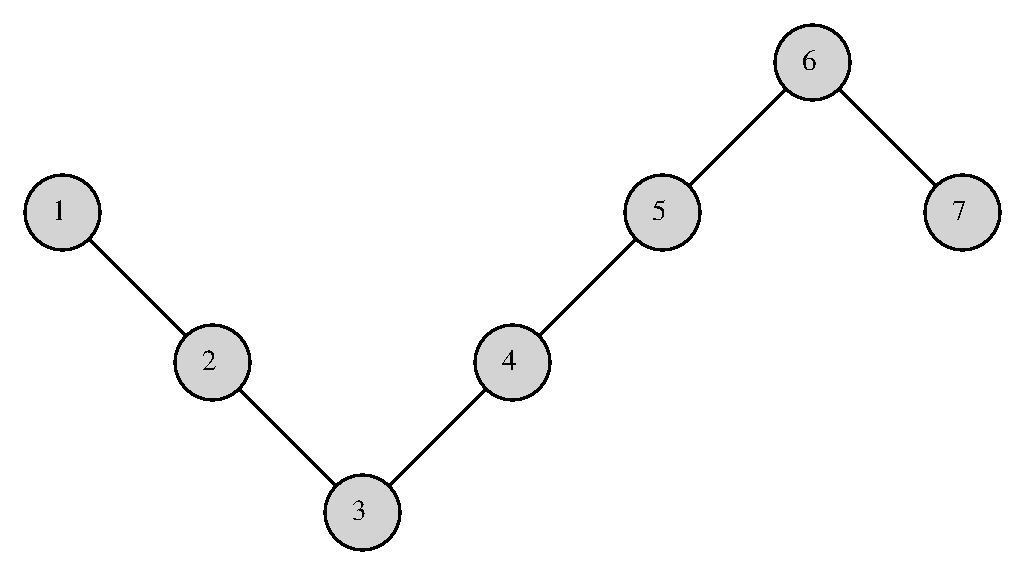
\includegraphics[scale=0.5]{./images/w-path.eps}}}%
    \qquad
    \subfloat[Monotone path decomposition of $P$, $P_1 = 1, 2, 3$, $P_2 = 3, 4, 5, 6$ and $P_3 = 6, 7$.]{{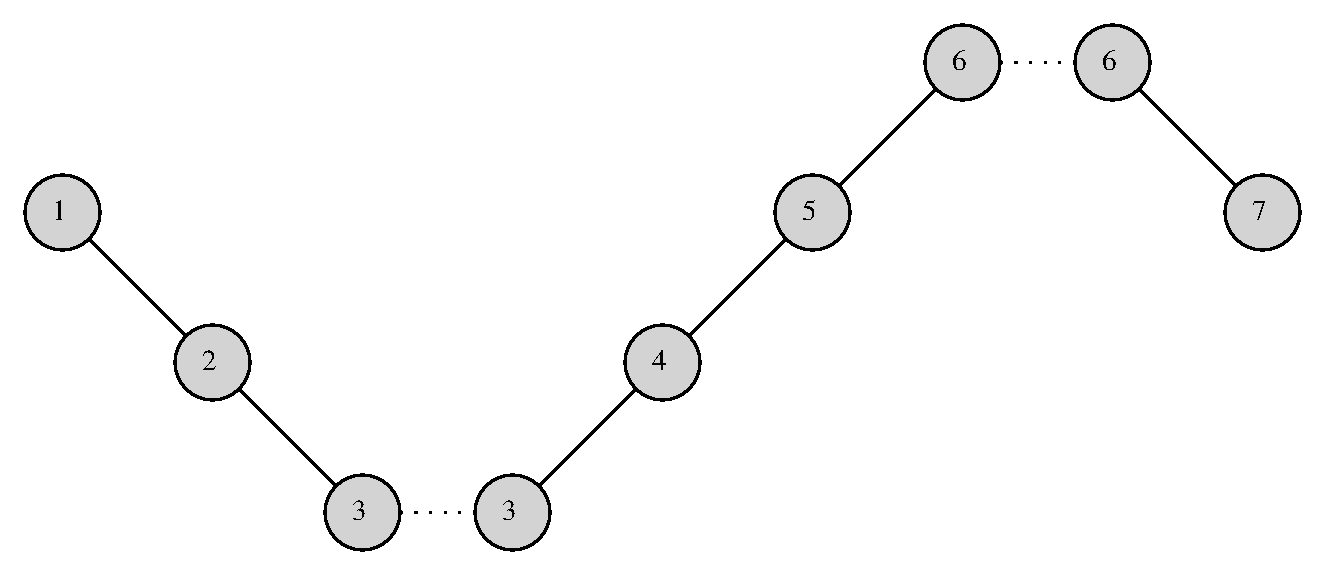
\includegraphics[scale=0.5]{./images/w-path-decomposed.eps}}}%
    \caption{A path and its monotone path decomposition.}
    \label{fig:monotone-decomposition}%
\end{figure}


%The maximum path with respect to this property is precisely the lower bound on the parallel algorithm introduced in []. As a special case we must note that paths that can be decomposed into less than four monotone paths do not pose an algorithmic problem.


A kink in a path is a vertex whose two neighbours are either both higher or both lower (Figure \ref{fig:a-tale-of-two-kinks}). Given the path $(u_1, u_2, ... , u_k)$ an inside vertex $u_i \ne u_1, u_k$ is a kink when $h(u_i) \notin \big( min(h(u_{i-1}),~h(u_{i+1})),~max(h(u_{i-1}),~h(u_{i+1})) \big)$. To avoid this cumbersome expression we shall adopt a slight abuse of notation and in the future write it as $h(u_i) \notin $ or $ \in $ $\big(h(u_{i-1}),~h(u_{i+1}) \big)$ where it will be understood that the lower bound of the interval is the smaller of the two and the upper bound the larger.

We can use the number of kinks in a path to define a metric on it. We will call this metric the w-length of a path and use it to measure the number of inside vertices of a path which are kinks. This is similar to how the length of a path is a metric that measures the number of edges between its vertices. The notation we will adopt for the w-length and length of a path $u \rightsquigarrow v$ is $w(u, v)$ and $d(u, v)$ respectively. There is no ambiguity here because as we have already said there is a unique path between any two vertices in a tree. One thing we can already claim is that $w(u, v) \le d(u, v)$ for any two vertices in a height tree. The length of a path with $n$ vertices is $n-1$, but at only the inside vertices of a path can be kinks. The number of inside vertices in a path of length $n \ge 2$ is $n - 2$.

\begin{figure}[h]%
    \centering
    \subfloat[Upwards kink.]{{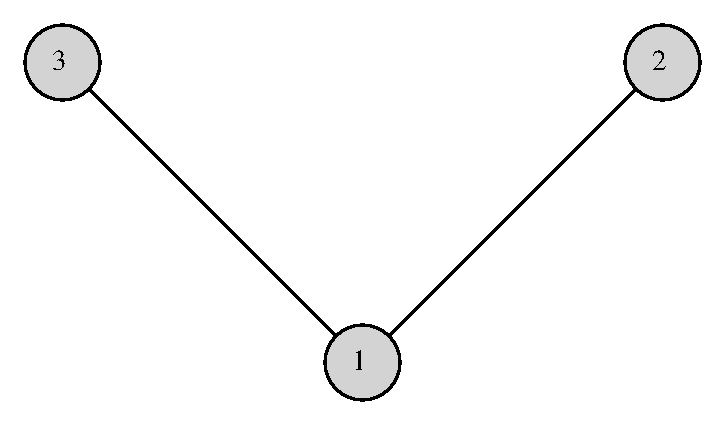
\includegraphics[scale=0.4]{./images/kinky-smile.eps}}}%
    \qquad \qquad \qquad
    \subfloat[Downwards kink.]{{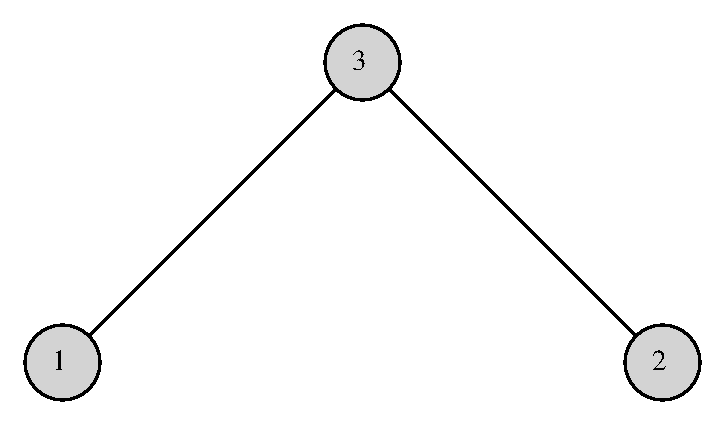
\includegraphics[scale=0.4]{./images/kinky-frown.eps}}}%
    \caption{Two possible types of kinks (vertices are labeled with their height).}%
    \label{fig:a-tale-of-two-kinks}%
\end{figure}


In Chapter 3 we foreshadowed our intention of obtaining the largest w-structure in a contour tree. We can now put this in more precise terms as the path in a height tree that has the maximum w-length (or the longest w-path). We can immediately obtain a brute force approach for this problem by considering all paths in the contour tree and computing their w-length to find the maximum one. This can be expressed with the following optimization term

\begin{equation}
    \label{eq:brute-force}
    \max_{u, v \in V(T)}\{ w(u, v) \} .
\end{equation}

The search space is quadratic in the number of vertices and measuring the w-length of a given path can be done by inspecting the height of every inside vertex and its two neighbours in the path. The worst case time complexity of this algorithm is $O(dn^2)$ where $d$ is the diameter (longest path) of the tree and $n$ is the number of vertices. This is far from satisfactory given that the worst case time complexity of the algorithm for computing the contour tree is close to linear. We can in fact do better.

In Chapter 2 we described two algorithms for obtaining the diameter of a tree. The analogy we made between w-length and length is that both are a metric on paths in a tree. Therefore it may be possible to modify those two algorithms to obtain the longest w-path instead of the longest path. We will call the longest w-path in a tree its w-diameter. Before showing how we can adapt the two tree diameter algorithms we need to establish the two key properties that will play a crucial role in proving the correctness of the two new algorithms.

%As the reader may have noticed the definitions we have made so far are analogous to the task of computing the longest path between any two vertices of a tree. This is completely intentional as we will demonstrate how algorithms for computing the longest path in a tree can be modified to produce the longest w-path instead. Finding the longest path of a graph in the general case is an \em NP-hard\em. Fortunately the Contour Tree is a tree. The longest path in a tree is known in the literature as it's diameter and has a polynomial time algorithm. The two most popular linear time algorithms found in the literature I will denote as Double Breadth First Search (2xBFS) and Dynamic Programming (DP). We will now take a look at how these algorithms work and hint at how they can be adapted in the next chapter.

% \section{Tree W-Diameter Algorithms}

%We will now step into the realm of w-detection. Before we outline the proposed algorithms we must establish two key properties which hold the difference between the tree diameter algorithms and their modification to tree w-diameter algorithms.


%We have introduced two tree diameter algorithms in the previous section. Let us now demonstrate how they can be adapted to the task of computing a height tree's w-diameter. Before doing so we need to establish the two key properties that will play a critiral part in adapting the algorithms.

\begin{defn} (Symmetry Property) Let $a \rightsquigarrow b$ be a path. Then $w(a, b) = w(b, a)$. \end{defn}

This property if true because the path $a \rightsquigarrow b$ contains the same vertices as the path $b \rightsquigarrow a$.

\begin{defn} (Subpath Property) Let $a \rightsquigarrow b$ be a path and $c \rightsquigarrow d$ its subpath. Then $w(a, b) \le w(c, d)$. \end{defn}

This property follows from the fact that all kinks of the path from $c$ to $d$ are also kinks of the path from $a$ to $b$. An important thing to note is that in the case of path length if one of the paths is a proper subpath of the other then the inequality is strict. This does not have to be the case with w-paths because the w-length decreases only when we reduce the number of kinks in the path.

\begin{defn} (Path Decomposition Property Property) Let $a \rightsquigarrow b$ be the path $(a, u_1, u_2, ..., u_k, b)$ and $u_i$ be an inside vertex for $i \in \{1, 2, ..., k\}$. Then \end{defn}

$$w(a, b) = w(a, u_i) + w(u_i, b) + w_{a \rightsquigarrow b}(u_i)$$
, where
$$
w_{a \rightsquigarrow b}(u_i) = \left\{
   \begin{array}{@{}l@{\thinspace}l}
       \text{0}  &: \text{if } h(u_i) \in \big(h(u_{i-1}),~h(u_{i+1}) \big) \text{ // $u_i$ is not a kink} \\
       \text{1} &: \text{otherwise // $u_i$ is a kink.} \\
   \end{array}
\right.
$$

To see why this property is true observe that $u_i$ can be a kink in the path from $a$ to $b$, but it cannot be a kink in the paths from $a$ to $u_i$ and from $u_i$ to $b$ because it is an endpoint of both. All other possible kinks besides $u_i$ are accounted for by either $w(a, u_i)$ or $w(u_i, b)$. Therefore when making use of path decomposition property we must account for whether the vertex we are decomposing a path at is a kink in that path or not.


\section{Linear Time Algorithm - 2xBFS}

Let us first explore how the Breadth First Search based tree diameter algorithm can be adapted to compute the w-diameter of a height tree. We will call the adaptation 2xBFS for short and it will follow exactly the same steps. The difference is that we will make a modificatin of the standard BFS algorithm. We will modifty if to compute w-distances from a given root vertex to all other vertices in the tree. The algorithm works by first running the modified BFS from any vertex in the height tree and then records the leaf that is farthest in terms of w-length. It then runs the modified BFS a second time from that vertex and again records the farthest vertex from it.

The pseudocode for this algorithm is presented in Algorithm 1. In the algorithm we use two properties of vertices. The property $u.d$ for $u \in V(T)$ is the w-distance of a vertex from the root and the property $u.\pi$ is the parent of a vertex in the modified BFS. We use the function $h(u)$ for the height of a vertex and we use the variable $furthest$ to record the furthest vertex from the root in terms of w-length. Note that because of the comparison u.d $\ge$ furthest.d the furthest vertex will always be a leaf of tree. This comparison forces us to break ties in w-distance with distance. Theoretically it does not have to, but it will simplify some of our notation and proofs. Therefore we will assume that the w-diameter in a height tree is always between two leaves.

\begin{algorithm}

\caption{Computing the W Diameter of a Height Tree.}

\begin{algorithmic}[1]

\Function{W\_BFS}{T, root}
    \State root.d = 0
    \State root.$\pi$ = root
    \State furthest = root

    \State Q = $\emptyset$
    \State Enqueue(Q, root)

    \While {Q $\ne \emptyset$}
        \State u = Dequeue(Q)

        \If {u.d $\ge$ furthest.d}
            \State furthest = u
        \EndIf

        \ForAll {v $\in$ $N(u)$}
            \If {v.$\pi$ == $\emptyset$}
                \State v.$\pi$ = u
                \If {h(u) $\notin$ \big(h(v),~h(u.$\pi$)\big)}
                    \State v.d = u.d + 1
                \Else
                    \State v.d = u.d
                \EndIf

                \State Enqueue(Q, v)

            \EndIf
        \EndFor
    \EndWhile
    \State Return furthest
\EndFunction

\Function{Calculate\_W\_Diameter}{T}
    \State s = <any vertex>
    \State u = W\_BFS(T, s)
    \State v = W\_BFS(T, u)
    \State return v.d
\EndFunction

\end{algorithmic}
\end{algorithm}



%\begin{lem} The Algorithm produces the endpoints of a path who is at most 2 kinks shy of being the kinkiest path in the tree. \end{lem}
This algorithm however is not guaranteed to produce an optimal solution. It may fail to produce the tree's w-diameter, but we can bound the error in terms of the w-diameter. The correctness of the algorithm is based on the following Lemma.

\begin{lem} The farthest leaf in terms of w-length from any vertex in a height tree is guaranteed to be the endpoint of a path whose w-length is at least that of the w-diameter minus two.
\label{lem:2xbfs-proof}
\end{lem}

\begin{proof}
Let $T$ be a height tree and $s \in V(T)$ be the initial vertex we start the first search at. After running the modified BFS twice we obtain two vertices $u$ and $v$ such that:

\begin{equation}
    \label{eq:su_all}
    w(s, u) \ge w(s, t), \forall t \in V(T),
\end{equation}

\begin{equation}
    \label{eq:uv_all}
    w(u, v) \ge w(u, t), \forall t \in V(T).
\end{equation}

Let $a$ and $b$ be two leaves that are the endpoints of a w-path whose length is that w-diameter of $T$. For any such pair we know that:

\begin{equation}
    \label{eq:ab_all}
    w(a, b) \ge w(c, d), \forall c, d \in V(T).
\end{equation}

By this equation we have that $w(a, b) \ge w(u, v)$. Our goal in this proof will be to give a formal lower bound on $w(u, v)$ in terms of $w(a, b)$. Let $t$ be the first vertex in the path between $a$ and $b$ that the first BFS starting at $s$ discovers. Note that $t$ cannot be $a$ or $b$ unless $s$ is equal to $a$ or $b$. The proof will be split into several cases depending on the relative positions of $s$, $t$, $a$, $b$ and $u$. \linebreak

{\em Case 1. When the path from $a$ to $b$ does not share any vertices with the path from $s$ to $u$.}

{\em Case 1.1. When the path from $u$ to $t$ goes through $s$.}

% @TODO Explain that the dotted lines are paths.
\begin{figure}[h]%
    \centering
    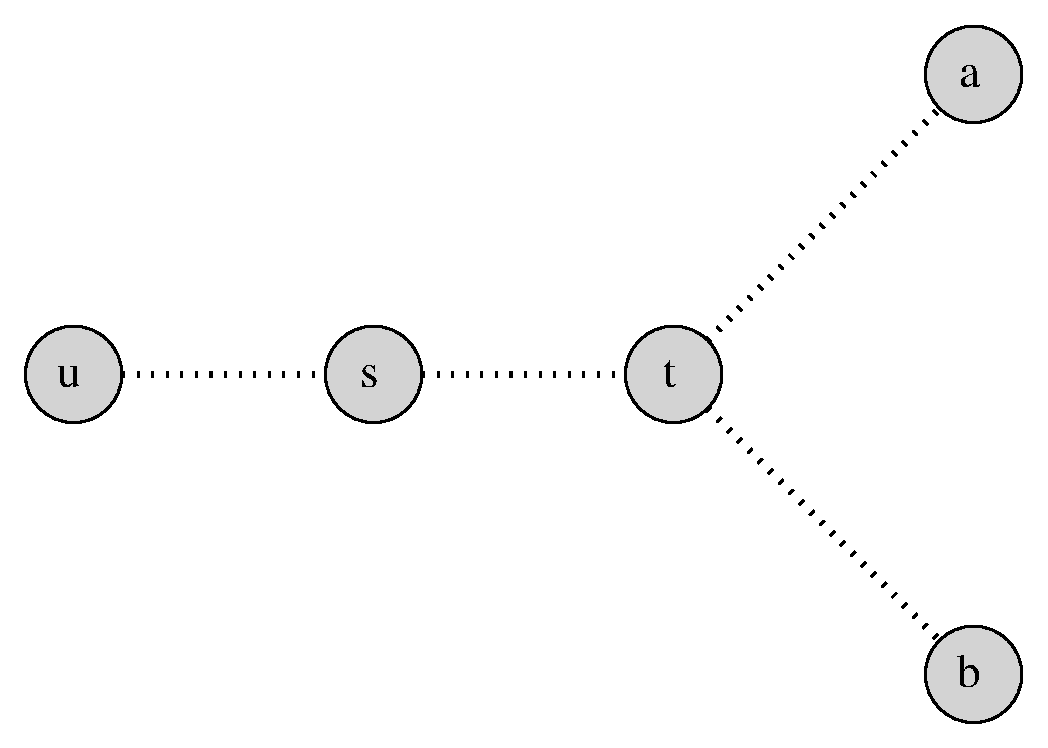
\includegraphics[center, scale=0.4]{./images/2xbfs-case-1-1.eps}
    \caption{Relative position of vertices in Case 1.1 (dotted lines are paths). }%
    \label{fig:case1.1}%
\end{figure}

In this case $s \rightsquigarrow u$ is a subpath of $t \rightsquigarrow u$. This means that $w(t, u) \ge w(s, u)$. By equation \ref{eq:su_all} we also have that $w(s, u) \ge w(s, a)$. We can therefore conclude that $w(t, u) \ge w(s, a)$. As $t \rightsquigarrow a$ is a subpath of $s \rightsquigarrow a$ then $w(s, a) \ge w(a, t)$. Upon combining these inequalities we obtain that $w(t, u) \ge w(a, t)$.


The vertex $t$ is a inside vertex for both the path $a \rightsquigarrow b$ and the path $u \rightsquigarrow b$. We can use the path decomposition property for both paths at $t$ as follows:
$$ w(a, b) = w(b, t) + w(t, a) + x  $$
$$ w(u, b) = w(b, t) + w(t, u) + y .$$
where $x = w_{a \rightsquigarrow b}(t)$ and $y = w_{u \rightsquigarrow b}(t)$. In other words $x, y \in \{0, 1\}$ depending on whether there is a kink at $t$ for the path from $a$ to $b$ and from $u$ to $b$ respectively. As $w(t, u) \ge w(a, t)$ we can show that:


$$ w(u, b) \ge w(b, t) + w(t, a) + y $$
$$ w(u, b) \ge w(b, t) + w(t, a) + x - x + y $$
$$ w(u, b) \ge w(a, b) - x + y $$
$$ w(u, b) \ge w(a, b) + (y - x) $$

But as $w(u, v) \ge w(u, b)$ (by equation \ref{eq:uv_all}) we obtain that:

$$ w(u, v) \ge w(a, b) + (y - x) $$

Considering all possible values that $x$ and $y$ can take, we can see that the minimum value for the right hand side of the inequality is at $y = 0$ and $x = 1$. This occurs when $t$ is a kink in the path from $a$ to $b$ but not a kink in the path from $u$ to $b$.

The final conclusion we may draw is that $w(u, v) \ge w(a, b) -1$.

{\em Case 1.2. When the path from $u$ to $t$ does not go through $s$.}

\begin{figure}[h]%
    \centering
    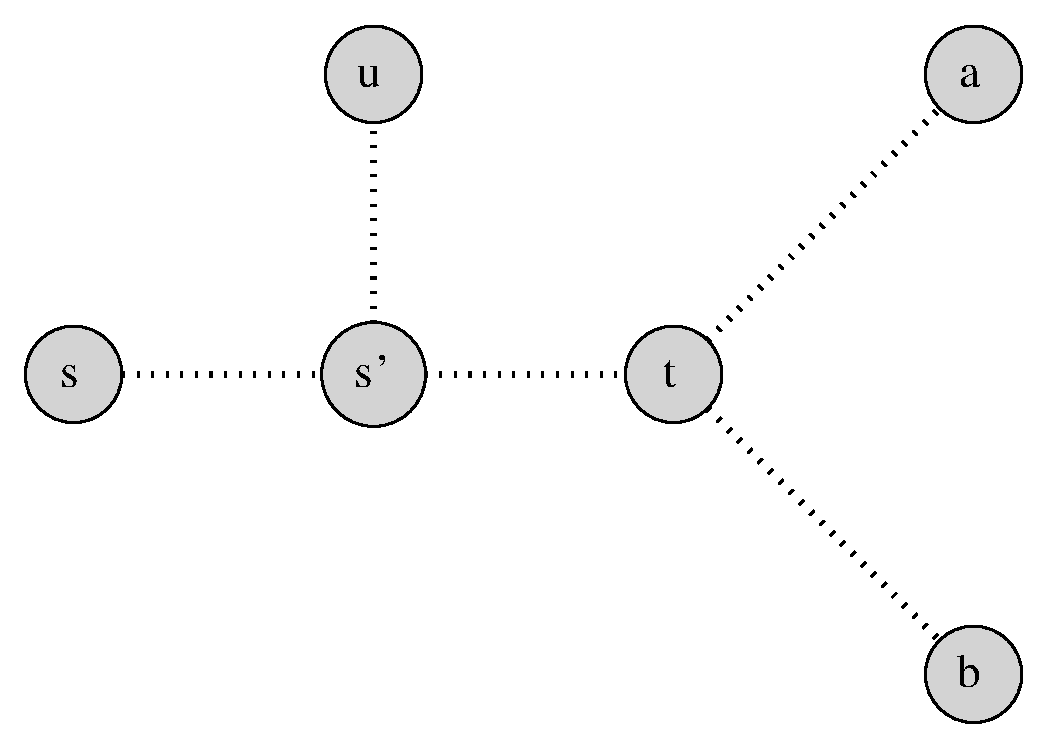
\includegraphics[center, scale=0.4 ]{./images/2xbfs-case-1-2.eps}
    \caption{Relative position of vertices in Case 1.2 (dotted lines are paths). }%
    \label{fig:case1.2}%
\end{figure}

If the path from $u$ to $t$ does not go through $s$ then the paths $s \rightsquigarrow t$ and $s \rightsquigarrow u$ have a common subpath. Let $s'$ be the last common vertex in that subpath. We will produce a proof that is similar to the previous case by considering $s'$ in the place of $s$. We must only account for whether $s'$ is a kink in one of the paths $s \rightsquigarrow u$ or $s \rightsquigarrow a$. Through path decomposition of $s \rightsquigarrow a$ and $s \rightsquigarrow u$ at $s'$ we obtain that:

$$ w(s, a) = w(s, s') + w(s', a) + x  $$
$$ w(s, u) = w(s, s') + w(s', u) + y, $$
where $x = w_{s \rightsquigarrow a}(s')$ and $y = w_{s \rightsquigarrow u}(s')$. By equation \ref{eq:su_all} we know that $w(s, u) \ge w(s, a)$ and therefore:

$$ w(s, s') + w(s', u) + y \ge w(s, s') + w(s', a) + x  $$
$$ w(s', u) + y \ge w(s', a) + x $$
$$ w(s', u) \ge w(s', a) + (x - y).$$

We know that $w(t, u) \ge w(s', u)$ because $s' \rightsquigarrow u$ is a subpath of $t \rightsquigarrow u$, so

$$ w(t, u) \ge w(s', a) + (x - y).$$

From the fact that $t \rightsquigarrow a$ is a subpath of $s' \rightsquigarrow a$ it follows that $w(s', a) \ge w(t, a)$. This allows us to infer that:

$$ w(t, u) \ge w(t, a) + (x - y). $$

Now we are ready to proceed in a similar manner as the previous case. We will decompose the paths from $b$ to $a$ and from $b$ to $u$ at the vertex $t$ as follows:

$$ w(b, a) = w(b, t) + w(t, a) + z  $$
$$ w(b, u) = w(b, t) + w(t, u) + w  $$
where $z = w_{b \rightsquigarrow a}(t)$ and $w = w_{b \rightsquigarrow u}(t)$. Then by $w(t, u) \ge w(t, a) + (x - y)$ we have that:

$$ w(b, u) \ge w(b, t) + w(t, a) + (x - y) + w $$
$$ w(b, u) \ge w(b, t) + w(t, a) + z - z + (x - y) + w $$
$$ w(b, u) \ge w(a, b) - z + (x - y) + w $$
$$ w(b, u) \ge w(a, b) + (x - y) + (w - z) .$$

The minimum value for the right hand side of this equation is at $x, w = 0$ and $y, z = 1$. Using the fact that $w(u, v) \ge w(u, b)$ we finally obtain $ w(u, v) \ge w(a, b) - 2 $.


{\em Case 2. When the path from $a$ to $b$ shares at least one vertex with the path from $s$ to $u$.}

\begin{figure}[h]%
    \centering
    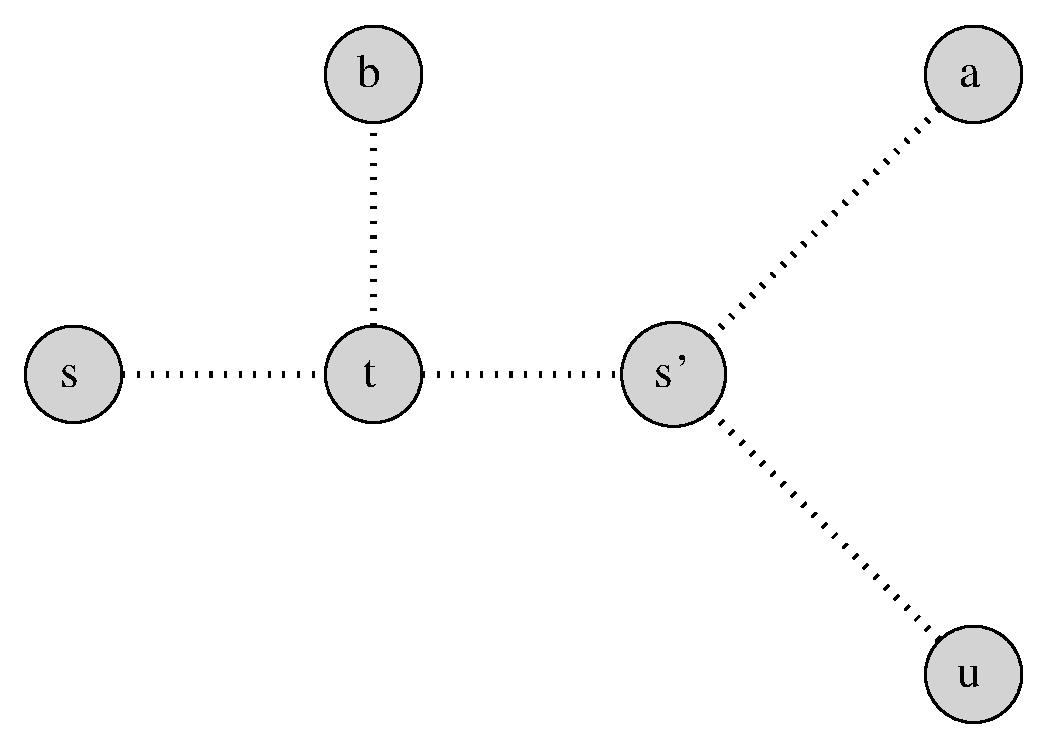
\includegraphics[center, scale=0.4 ]{./images/2xbfs-case-2.eps}
    \caption{Relative position of vertices in Case 2 (dotted lines are paths). }%
    \label{fig:case2}%
\end{figure}

% @TODO This is not complete!
%As we already know $w(s, u) \ge w(s, a)$. Furthermore $w(s, u) \ge w(t, u)$ and $w(s, a) \ge w(t, a)$ as they are subpaths of $s \rightsquigarrow u$ and $s \rightsquigarrow a$ respectively. Therefore $w(t, u) \ge w(t, a)$. We can now decompose the paths from $b$ to $a$ and from $b$ to $u$ at the vertex $t$ as follows:

We can do a path decomposition as follows:

$$ w(s, u) = w(s, t) + w(t, u) + x $$
$$ w(s, a) = w(s, t) + w(t, a) + y $$
where $x = w_{s \rightsquigarrow u}(t)$ and $y = w_{s \rightsquigarrow a}(t)$. As $w(s, u) \ge w(s, a)$ (by equation \ref{eq:su_all})we obtain that:

$$ w(s, t) + w(t, u) + x  \ge w(s, t) + w(t, a) + y $$
$$ w(t, u) \ge w(t, a) + (y - x) $$

If we again decompose the paths from $b$ to $a$ and from $b$ to $u$ at $t$ we obtain:

$$ w(b, a) = w(b, t) + w(t, a) + z  $$
$$ w(b, u) = w(b, t) + w(t, u) + w  $$
where $z = w_{b \rightsquigarrow a}(t)$ and $w = w_{b \rightsquigarrow u}(t)$. Then by $w(t, u) \ge w(t, a) + (x - y)$ we have that:

$$ w(b, u) \ge w(b, t) + w(t, a) + (x - y) + w $$
$$ w(b, u) \ge (w(b, t) + w(t, a) + z) - z + (x - y) + w $$
$$ w(b, u) \ge w(a, b) - z (x - y) + w $$
$$ w(b, u) \ge w(a, b) + (x - y) + (w - z). $$

Where similarly to the previous case the rightful conclusion is that $ w(u, v) \ge w(a, b) - 2 $.

Based on these cases we have shown that that for any input tree the algorithm will produce a w-path that is at most two kinks less than the actual w-diameter of the tree.

\end{proof}

Let us now show some formal bounds on the time and space complexity of the 2xBFS algorithm.

\begin{lem} The time complexity of the algorithm is $O(|V|)$. \end{lem}

\begin{proof}
    The modified BFS function has the same time complexity as BFS. All we have added to the standard BFS is an "\em if, then, else\em"~statement. The time complexity of BFS is $O(|V| + |E|)$, but in a tree $|E| = |V| - 1$, so the overall complexity is $O(2|V| - 1) = O(|V|)$.
    Running the modified BFS function a second time only adds a linear factor the expression and thus the overall complexity of the algorithm is linear.
\end{proof}

\begin{lem} The space complexity of the algorithm is $O(|V|)$. \end{lem}

\begin{proof}
    The modified BFS function has the same space complexity as the standard BFS. Therefore the space complexity of 2xBFS is $O(|V|)$.
\end{proof}

\subsection{Pathological Cases in 2xBFS}

Here we will present some examples of pathological cases where the w-diameter outputted by the 2xBFS algorithm differs from the actual w-diameter (Figure \ref{fig:path-cases}). Each one of the examples corresponds to one of the cases in Lemma \ref{lem:2xbfs-proof}. In all examples the initial vertex is taken to be $s$. We have that $w(s, u) = w(s, a) = w(s, b) = 1$, but $d(s, u) > d(s, a) = d(s, b) = 1$. This ensures that $u$ is the last vertex with w-distance $1$ visited from the modified BFS. After running the algorithm the vertex outputted by the first BFS function is $u$. After running the second BFS the longest w-path would be $u \rightsquigarrow a$ or $u \rightsquigarrow b$. We can see that in all figures $w(u, a) = w(u, b) = 1 \text{ or } 2$, but $w(a, b) = 3$.

% Even if we adapt the algorithm so that it finds the vertex with that is farthest in terms of both w-length and length we will still be able to make simillar pathological case examples. We just need to augment the height trees by making $u$ further away from $s$ that $a$ and $b$ but keeping the same relative w-length of all paths.

\begin{figure}[h]%
    \centering

    \subfloat[Pathological Example for Case 1.1 (-1 of actual w-diameter).]{{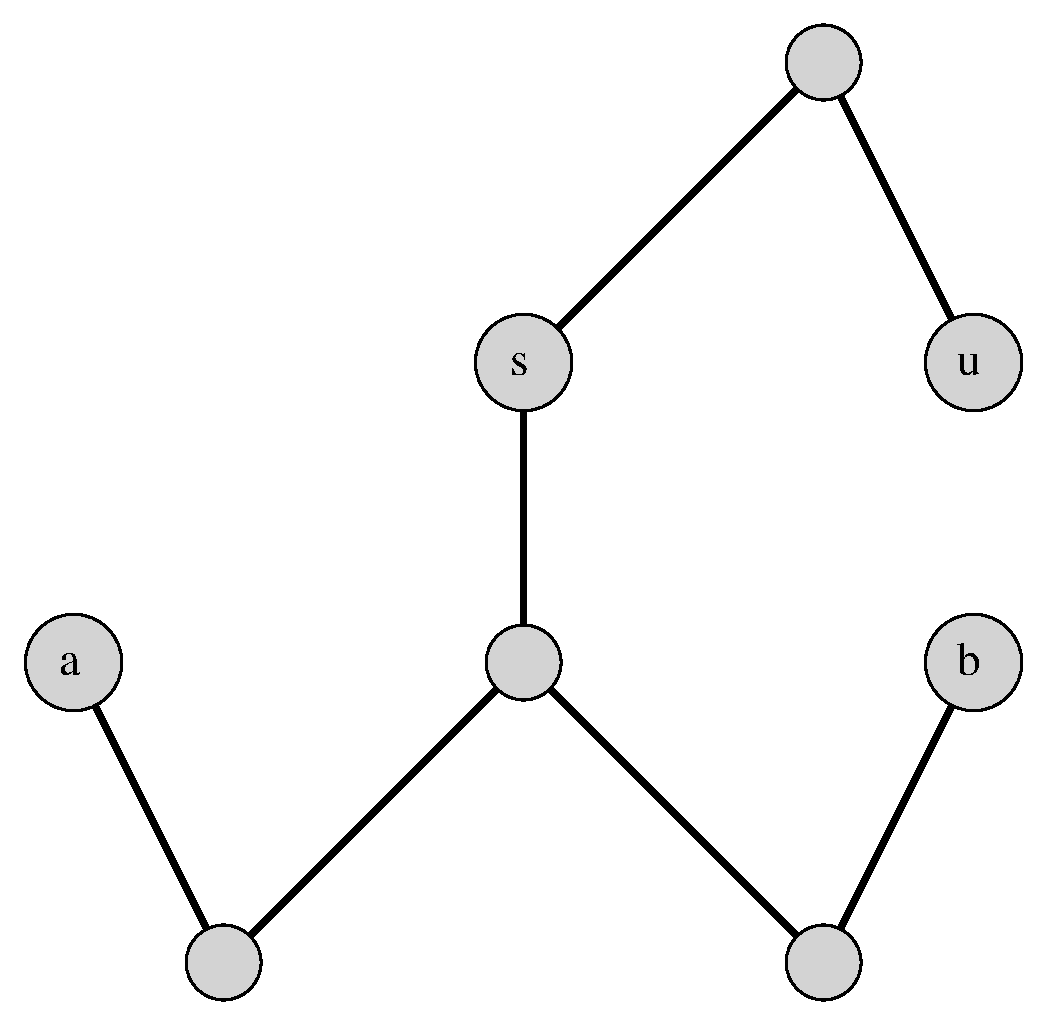
\includegraphics[scale=0.3]{./images/2xbfs-path-case-1-1.eps}}}%
    \qquad
    \subfloat[Pathological Example for Case 1.2 (-2 of actual w-diameter).]{{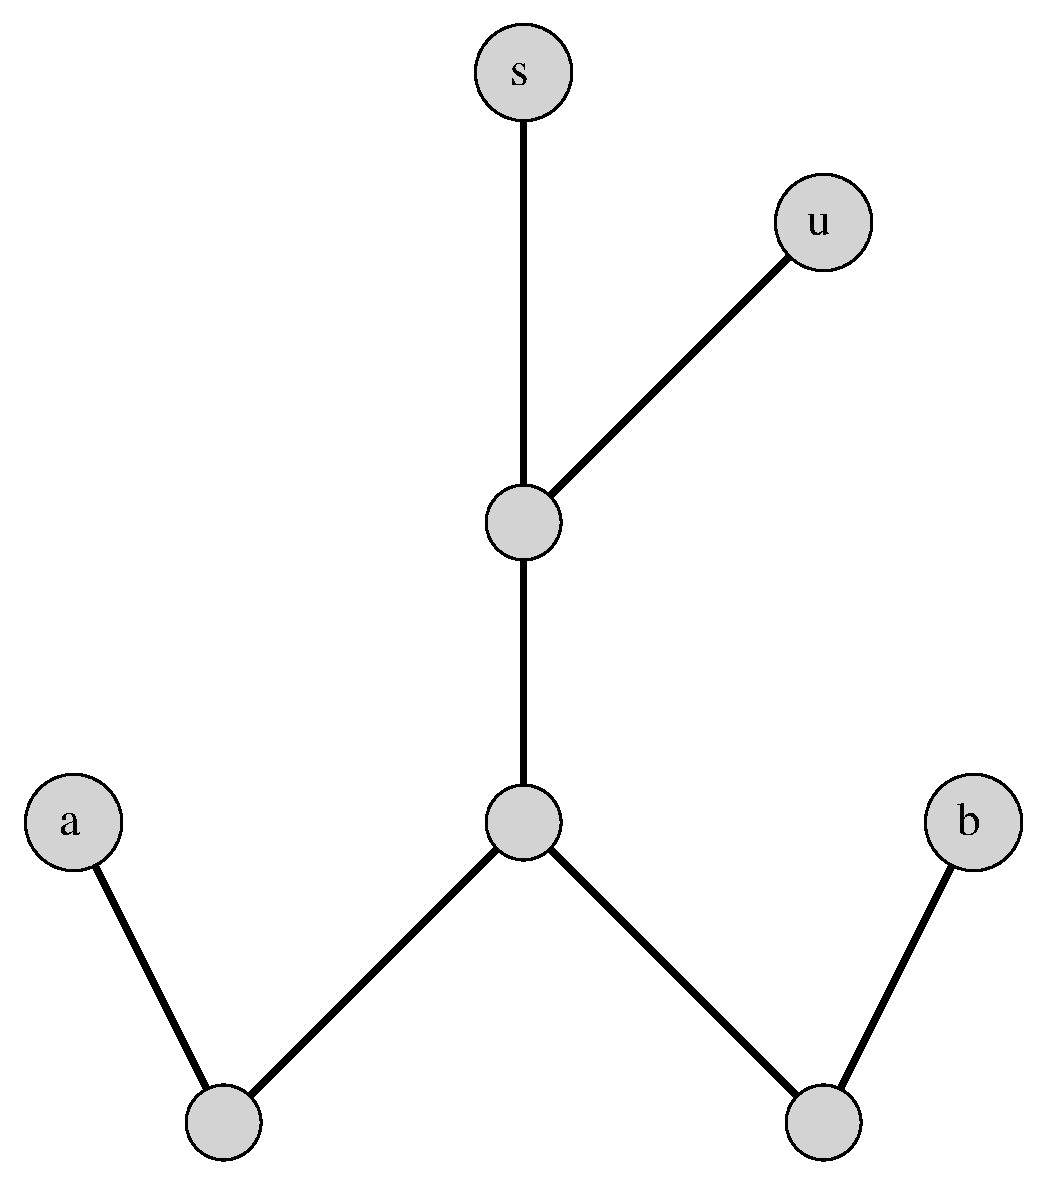
\includegraphics[scale=0.3 ]{./images/2xbfs-path-case-1-2.eps}}}%
    \qquad
    \subfloat[Pathological Example for Case 2 (-2 of actual 2-diameter).]{{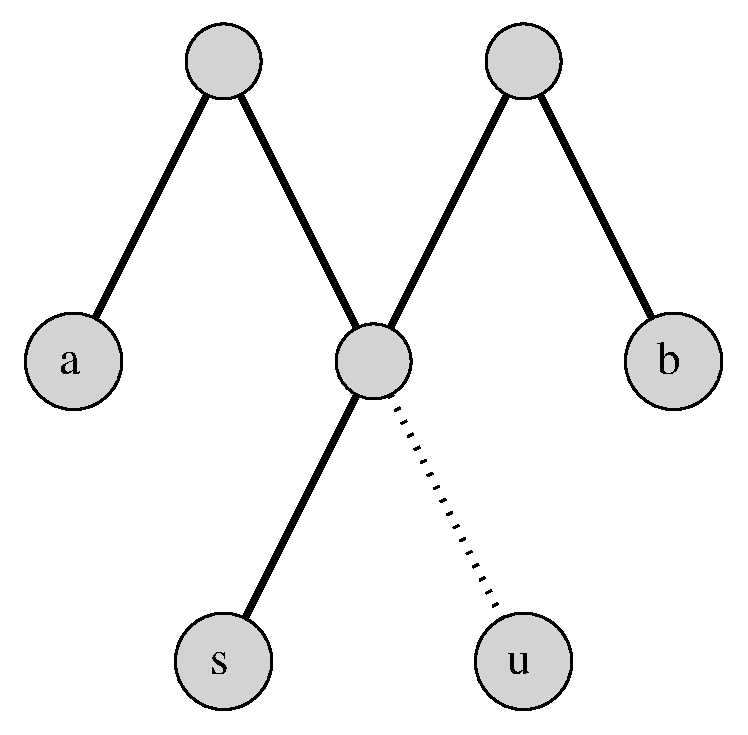
\includegraphics[scale=0.3 ]{./images/2xbfs-path-case-2.eps}}}%
    \caption{Pathological cases in the 2xBFS algorithm (dotted lines are \textbf{monotone} paths of length at least three).}%
    \label{fig:path-cases}%
\end{figure}

If we modified the algorithm to output the closest vertex to the root with maximum w-distance we would obtain the correct output on these example. If however we replace the dotted monotone path with a single edge then $u$ becomes the closest vertex to $s$ and as such will be the one outputted by the first BFS. In that case the algorithm will still output smaller w-path than the w-diameter.


\subsection{Attempts at resolving the accuracy of 2xBFS}


%For the intents and purposes of this dissertation the accuracy of this algorithm is sufficient. In large enough data sets this estimate provides enough insight to correlate the observed iterations needed to collapse the split and join trees and the resulting w-diameter of the tree. This is demonstrated empirically in Chapter 3. Regardless of such practical considerations it is still of inherent theoretical interest to investigate how we may be able to obtain a more accurate modification of this algorithm.

% In this section we adapted the first of the tree diameter algorithms to obtain a w-diameter algorithm with what we claim is reasonable accurate. That accuracy is supported by Lemma [], but we have not way of knowing whether the w-path obtained through 2xBFS is optimal of not. Here we will present two possible ways of improving the accuracy of the output of the 2xBFS algorithm and explain why were not able improve upon the theoretical bound of Lemma [].

Here we will present two possible ways of improving the accuracy of the output of the 2xBFS algorithm and explain why were not able improve upon the theoretical bound of Lemma \ref{lem:2xbfs-proof}.

One key observation we can make is that on the second run of the BFS we get a w-path that is necessarily longer or equal to one found in the first BFS search. A natural question to ask is whether running the BFS a third, fourth or for that matter nth time would result in the actual w-diameter. On every successive iteration we get a w-path that is longer or equal to the previous one, because w-length is a symmetric path property ($w(a, b) = w(b, a)$). By doing this we can hope that we will eventually obtain a w-path closer to the w-diameter. However there is no guarantee that this will happen. In some cases it is possible that each successive BFS returns the same path over and over again. As an example consider Figure \ref{fig:case3}. If the algorithm starts at $s$ then every successive iterrations will go between $u$ and $v$ and then $v$ and $u$ and so on.
This is because $w(u,v) > w(u, a) = w(u, b)$ and $w(v, u) = w(v, a) = w(v, b)$, but $d(v, u) > d(v, a) = d(v, b)$.

\begin{figure}[h]%
    \centering
    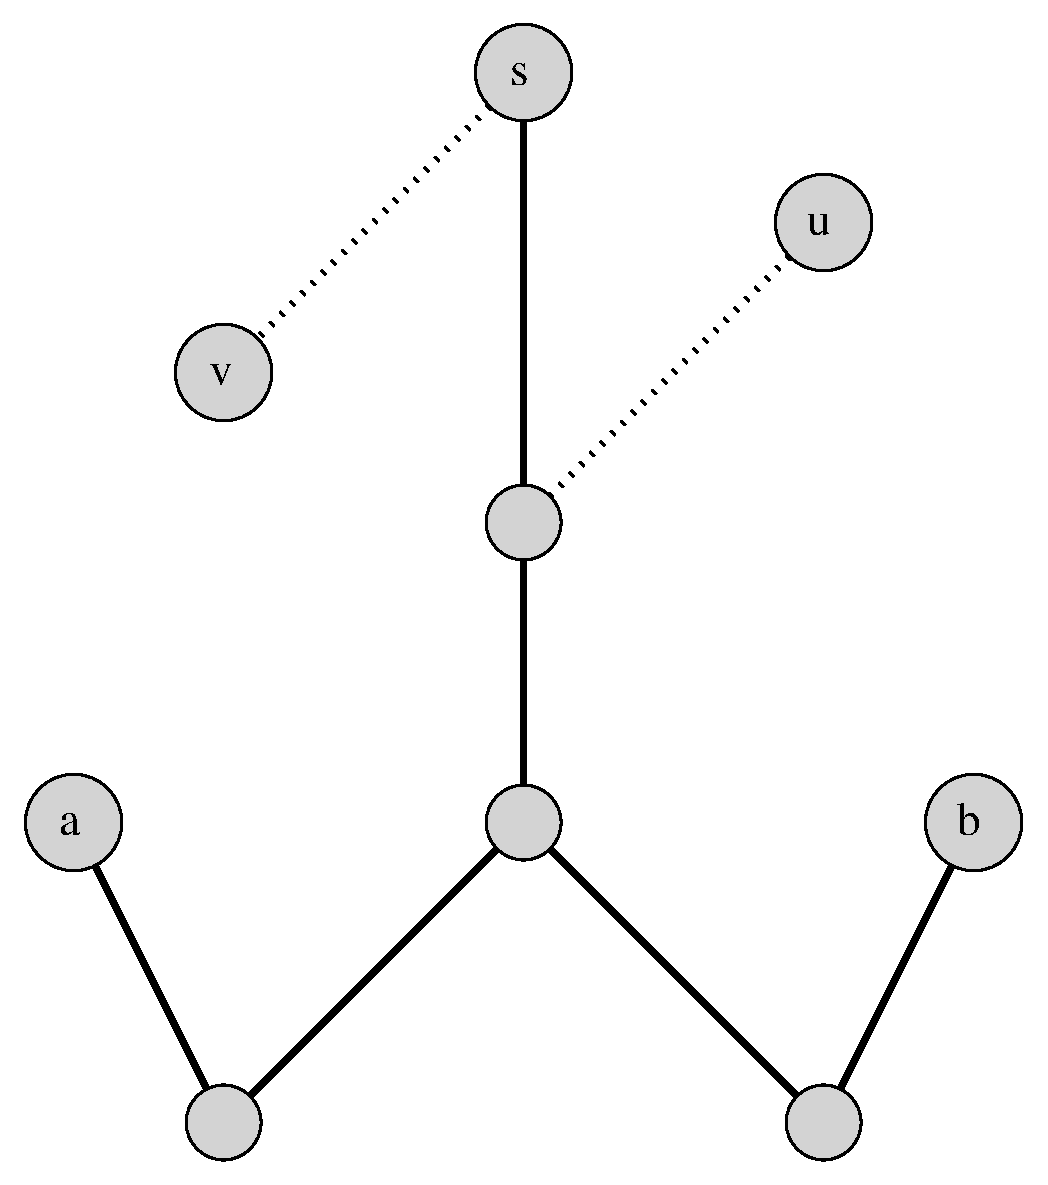
\includegraphics[center, scale=0.3]{./images/2xbfs-path-case-3.eps}
    \caption{Infinite cycle between $u$ and $v$ (dotted lines are monotone paths of length at least 3). }%
    \label{fig:case3}%
\end{figure}

% Obverse how in Figure [] all iterations of BFS go from the vertex $u$ to the vertex $v$ and then from $v$ to $u$ and so on.

A different heuristic we can apply is to run the algorithm multiple times from different starting vertices and keep the maximum value found. This approach is most reliable when we run the algorithm from all vertices in the tree. The we will obtain the obtain the w-diameter. The issue in doing so is that the time complexity will become quadratic and we would be no better off than with the exhaustive brute force approach. If however we run the algorithm for some subset of the vertices in the tree we lose all guarantees on the accuracy. There may simply be too few vertices from which the algorithm would obtain the actual w-diameter.




%In the search for a better solution let $s$ be a starting vertex and let the vertices $U = \{u_1, u_2, ..., u_n\}$ be the furthest away in terms of w-distance and $W = \{w_1, w_2, ..., w_n\}$ be the ones second furthest away. By the proof of the algorithm we know that not necessarily all vertices in those sets would produce a w-diameter. Thus lets us define $R \subseteq U \cup W$ as the set of vertices which are endpoints of a w-diameter. As we have shown we can construct an example where $|R| = 2$ and $|U \cup W|$ is arbitrarily large. Can we then find some property of the vertices in $R$ and pick them out in the first phase of the algorithm? *This I will leave open for the future generations to ponder. I hope in doing so all people of the world will unite unite and end all wars and prejudices in order to work towards this common good!*

\section{Dynamic Programming Algorithm - DP}

It is encouraging that we have obtained an algorithm that bounds the w-diameter but it is also unsatisfactory that we were not able to directly obtain it. To remedy this we will resort to modifying the second tree diameter algorithm. We will use the same optimisation strategy i.e. dynamic programming by making two key changes. Instead of the function $h(u)$ that stores the height of a subtree with root $u$ we will use the function $w(u)$ that stores the longest w-path that starts at the root of the subtree (the w-height). We will rename the function that stores the value of the optimal solutions for subroblems from $D(u)$ to $W(u)$ accordingly. To summarise $W(u)$ returns the length of the largest w-path in the subtree $T_u$ and $w(u)$ the length of the largest w-path in $T_u$ that starts at $u$. Note also that in the case of rooted trees we define $N(u)$ to not include the parent of $u$.

%This may seem like a simple substitution at first glance, but the devil is in the details.
Similarly to the modification of the BFS based algorithm all additional difficulties stem from the difference in the properties of length and w-legnth of paths. Let us first define the w-height of rooted height tree. It is the longest w-path that starts at the root of the tree. We will now examine how w-height can be computed in manner similar to the height of a rooted tree. Let $T$ be a rooted tree and $s \in V(T)$ be any vertex. Let us also assume the we have computed the w-heights of the children of $s$. In the case of computing the height we can simply set $h(s) = \max\limits_{u \in N(s)}\big( h(u) \big) + 1$. We cannot do so with the w-height because w-length can remain the same if we do not extend the maximum w-path with a kink.  To demonstrate this let us assume that $u \in N(s)$ is such that $w(u) = \max\limits_{v \in N(s)}(w(v))$. Then if we wish to extend the maximum w-path that ends at $u$ to $s$ we must account for whether $u$ becomes a kink in it. If none of the children of $s$ with maximum w-height form a kink when extending to $s$ then the w-height of $s$ does not increase.

In order to obtain the w-height of $s$ let $u$ be any of its children and $L_u = \{u_1, u_2, ..., u_k\}$ be all children of $u$ through which a w-path with length $w(u)$ passes through. We can compute the w-height of $s$ as follows: $w(s) = \max\limits_{u \in N(s)}\{ w(u) + \max\limits_{v \in L_u}(w_{s \rightsquigarrow v}(u)) \}$. In other words there may be multiple w-paths with the same maximal w-length that end at $u$. If possible we must pick the one that would make $u$ form a kink with $s$. If not we can use any of them. It is of no use to consider paths of lesser w-length because when adding $s$ to them the w-length may increase by at most one and match any of maximal paths that go through a vertex in $L_u$.

The second ingredient in the dynamic programming approach of the tree diameter algorithm was to combine the two longest paths that end at children of the root of the subtree (height paths). As before let $T$ be a tree and $s$ be its root. We first find two distinct children $u, v \in N(s)$ of $s$ such that $h(u)$ and $h(v)$ is maximum amongst all children and $u \ne v$ (otherwise we do not get a proper path). Next we will combine the height paths of $u$ and $v$ in order to obtain the longest path that goes through $s$. The length of this new path is given by the summation $h(u) + h(v) + 2$. The $2$ is added to account for the two additional edges $us, sv \in E(T_s)$. This method of combining paths of course extends to all subtrees in $T$.

In the case of w-path combinations we must be vigilant of which vertices become kinks in the path combinations. Let us observe a similar scenario where $s$ is the root of a rooted tree height $T$ and $u, v \in V(T_s)$ are two of the children with maximal values for $w(u)$ and $w(v)$. We would ideally like to combine $w(u)$ and $w(v)$ like so: $w(u) + w(v) + w_{u, v}(s)$. This however is not correct. There is a hidden assumption in the sum that the only vertex that can become a kink in this path combination is $s$. Contrary to this, in fact $u$ and $v$ can also become kinks. Observe that $w(u) \text{ and } w(v)$ are the w-lengths of two paths. One path starting at $u$ and ending in a leaf of $T_u$ and one starting at $v$ and ending in a leaf of $T_v$. In the new path both $u$ and $v$ become inside vertices and depending on whether they become kinks or not the sum may further increase by two. To account for this we must also look at the children of $u$ and $v$ through which a maximum w-path passes. We have already introduced those as $L_u$ and $L_v$. This process is similar to the one for obtaining the w-height of a vertex and is described by the following formula:

$$ \max\limits_{\substack{u, v \in N(s) \\ u \ne v}}\bigg( h(u) + \max\limits_{t \in L_u}\Big(w_{s \rightsquigarrow t}(u)\Big) + h(v) + \max\limits_{t \in L_v}\Big(w_{s \rightsquigarrow t}(v)\Big) + w_{u \rightsquigarrow v}(s)\bigg). $$

The longest w-path in a rooted height tree is either entirely contained in one of the subtrees of the root or is a combination of two maximum w-height paths that end at two distinct children of the root. Attention must be paid to one special case. This is when the root of a rooted height tree has exactly one child. We cannot make a path combination in that case so we will use the w-height instead. By combining what we have shown so far we obtain the following expression for the optimal solution:

% $$ W(s) = \max\Bigg\{ \max\limits_{u \in N(s)}\bigg(W(u)\bigg), \max\limits_{\substack{u, v \in N(s) \\ u \ne v}} \bigg( h(u) + \max\limits_{t \in L_u}\Big(w_{s \rightsquigarrow t}(u)\Big) + h(v) + \max\limits_{t \in L_v}\Big(w_{s \rightsquigarrow t}(v)\Big) + w_{u \rightsquigarrow v}(s) \bigg), \max\limits_{u \in N(s)} \bigg( h(u) + \max\limits_{t \in L_u}\Big(w_{s \rightsquigarrow t}(u)\Big) \bigg) \Bigg\}. $$


$$
W(s) = \max\left\{
   \begin{array}{@{}l@{\thinspace}l}
       \max\limits_{u \in N(s)}\bigg(W(u)\bigg), \\
       \max\limits_{u \in N(s)} \bigg( h(u) + \max\limits_{t \in L_u}\Big(w_{s \rightsquigarrow t}(u)\Big) \bigg), \\
       \max\limits_{\substack{u, v \in N(s) \\ u \ne v}} \bigg( h(u) + \max\limits_{t \in L_u}\Big(w_{s \rightsquigarrow t}(u)\Big) + h(v) + \max\limits_{t \in L_v}\Big(w_{s \rightsquigarrow t}(v)\Big) + w_{u \rightsquigarrow v}(s) \bigg). \\
   \end{array}
\right.
\label{eq:uv_all}
$$

We will prove the correctness of the algorithm with the following Lemma.

\begin{lem} The computation for the longest w-path that goes through the root of a subtree is correct. \end{lem}
\begin{proof}

   Let $T$ be a rooted height tree and $s$ be its root.

   \em Case 1. $s$ has one child. \em

   When $s$ has exactly one child then the w-length of the longest path that goes through $s$ is equal to the w-height of $s$ by the definition of w-height.

   \em Case 2. $s$ has more than one child. \em

   Let $u', v' \ne s$ be two distinct leaves of $T$ such that the path $u' \rightsquigarrow v'$ is the longest w-path that goes through $s$.
   We can decompose the path $u' \rightsquigarrow v'$ at $s$ as: $w(u', v') = w(u', s) + w(v', s) + w_{u' \rightsquigarrow v'}(s)$.

   Let $u$ and $v$ be the two children of $s$ through which the path $u' \rightsquigarrow v'$ goes through.
   The paths $w(u', s)$ and $w(v', s)$ can be further decomposed at $u$ and $v$ respectively. We obtain that
   $w(u', s) = w(u', u) + w(u, s) + w_{u' \rightsquigarrow s}(u)$ and
   $w(v', s) = w(v', v) + w(v, s) + w_{v' \rightsquigarrow s}(v)$.
   In both cases $w(v, s) = 0$ and $w(u, s) = 0$ because $u$ and $v$ are adjacent to $s$. This means that the paths $u \rightsquigarrow s$ and $v \rightsquigarrow s$ have no inside vertices.
   Lastly we have that $w_{u' \rightsquigarrow v'}(s) = w_{u \rightsquigarrow v}(s)$ because $u \rightsquigarrow v$ is a subpath of $u' \rightsquigarrow v'$ and both contains $s$.
   By substituting these into the first equation we obtain that:

   $$w(u', v') = w(u', u) + w_{u' \rightsquigarrow s}(u) + w(v', v) + w_{v' \rightsquigarrow s}(v) + w_{u \rightsquigarrow v}(s). $$

   This equation is similar to the expression for the optimal solution. By observing the two carefully we can infer that
   $$w(u', u) + w_{u' \rightsquigarrow s}(u) = h(u) + \max\limits_{t \in L_u}\Big(w_{s \rightsquigarrow t}(u)\Big)$$
   and
   $$w(v', v) + w_{v' \rightsquigarrow s}(v) = h(v) + \max\limits_{t \in L_v}\Big(w_{s \rightsquigarrow t}(v)\Big).$$
   for otherwise we would be able to assemble a longer w-path that goes through $s$. This is not possible because we supposed that $u' \rightsquigarrow v'$ is the longest such w-path. Therefore we can conclude that:

   $$ w(u', v') \le \max\limits_{\substack{u, v \in N(s) \\ u \ne v}}\{ h(u) + \max\limits_{t \in L_u}\Big(w_{s \rightsquigarrow t}(u)\Big) + h(v) + \max\limits_{t \in L_v}\Big(w_{s \rightsquigarrow t}(v)\Big) + w_{u \rightsquigarrow v}(s)\}. $$

   The w-path combination on the right hand side of this inequality is valid path in the tree that goes through $s$. It follows that it cannot be strictly bigger than $w(u', v')$. Therefore they are equal and the computation produces the longest w-path that goes through the root of the tree.

   \end{proof}

\begin{lem} The DP algorithm produces the w-diameter of a height tree. \end{lem}

\begin{proof}

   We just showed the longest w-path through the root of subtree is computed correctly. As the value of the optimal solution is taken in the same way as in the dynamic programming tree diameter algorithm then the correctness of our algorithm follows directly from it.

\end{proof}

The pseudocode of the proposed w-diameter algorithms is shown in Algorithm 2. The algorithm uses the following arrays:

\begin{itemize}
    \item W[u] - stores the value of the optimal solution.
    \item h[u] - stores the w-height.
    \item L[u] - stores a list of all children through which a w-height path passes.
    \item u.$\pi$ - stores the parent of a vertex (or itself if is the root).
\end{itemize}

The algorithm is a modification of the standard DFS algorithm. In the forward phase of the DFS we set the parents of all vertices in order to root tree and sets the optimal solution to all leaves to 0 as they are bases cases. In the backtracking phase of the algorithm was know that all children of the vertex we are at have been solved for. This is where we implement the recursive formula we developed. The steps of the algorithm are described via comments in the pseudocode.

% The steps are the following. Suppose that the current vertex is $s$.

% \begin{itemize}
%     \item Find all children $u$ of $s$ with maximum w-height and populate their list of children L[u].
%     \item Find the two children of $s$ whose w-height path combinations is maximal.
%     \item Find a child $u$ of $s$ whose value for the optimal solution W[u] is maximal.
%     \item Output maximum of W[u] and the maximum w-height path combination found.
% \end{itemize}

Next we will show a formal bound on the space complexity of the algorithm.

\begin{lem} The space complexity of the DP algorithm is $O(|V|)$. \end{lem}

\begin{proof}
    The sizes of all arrays we use in the algorithm is linear in the size of the tree. Therefore the space complexity of DP is $O(|V|)$.
\end{proof}

Let us provide formal bounds on the time and space complexity of the proposed solution. We can summarise the time complexity in the following formula:

$$ O\bigg( |V| + |E| + \sum_{u \in V}{\sum_{v \in N(u)}{d(v)}} + \sum_{u \in V}{d(u)^2}  \bigg) ,$$
where we use $d(u)$ for the degree of a vertex. The term $|V| + |E|$ comes from executing the Depth First Search, the term $\sum_{u \in V}{\sum_{v \in N(u)}{d(v)}}$ is the nested double loop over all children of children of all vertices (on line 15 and 22) and $\sum_{u \in V}{d(u)^2}$ is the nested double loop over all children in the final path combination (on line 31). We will begin by showing that

$$ O\bigg( \sum_{u \in V}{\sum_{v \in N(u)}{d(v)}} \bigg) = O(|V|) .$$

When running DFS on a tree it is not possible to visit a vertex as a child of a child more than once. Suppose for the sake of contradiction that it were possible. Let $T$ be a height tree and suppose we execute DFS to root $T$ from the vertex $s$. Let and $u, v$ be two distinct vertices such that the vertex $t$ is a child of a child of both. Then $s \rightsquigarrow u \rightsquigarrow t \rightsquigarrow v \rightsquigarrow s$ is a cycle in $T$. Trees have no cycles so this is a contradiction.

Let us now move on to the last term $\sum_{u \in V}{d(u)^2}$. We can immediately bound it from bellow via the inequality $ \sum_{u \in V}{d(u)^2} \ge \sum_{u \in V}{d(u)} = 2|E|$. This inequality holds because the degree of a vertex is a positive integer and for any $x \in Z^+$ $ x^2 \ge x$. Let us now show how it can be bounded from above.

A triangle is a complete graph on three vertices. Trees have no cycles thus they cannot have induced triangles. Therefore for any edge in a tree $uv \in E(T)$ we have that $d(u) + d(v) \le |V|$. If there were a vertex $t$ that is in both $N(u)$ and $N(v)$ then $uv, tu, tv \in E(T)$ would be an induced triangle which is a contradiction. If we use this to sum over all edges we obtain that:

$$ \sum_{uv \in E(T)}{d(u) + d(v)} \le |E||V|. $$

The key to transforming this inequality is to expand the summation $\sum_{uv \in E(T)}{d(u) + d(v)}$. When it is expanded every term $d(u)$ will be present exactly $d(u)$ times. One time for each one of its adjacent edges and there are exactly $d(u)$ adjacent edges. Therefore:

$$ \sum_{u \in V(T)}{d(u)^2} = \sum_{uv \in E(T)}{d(u) + d(v)} \le |E||V| .$$

To summarise what we have obtained so far:

$$ O\bigg( \sum_{u \in V}{\sum_{v \in N(u)}{d(v)}} \bigg) = O(|V|)  , ~~ O\bigg( \sum_{u \in V(T)}{d(u)^2} \bigg) = O(|V||E|).$$

Therefore a upper bound on the worst case time complexity of our dynamic programming solution is:

$$ O\big( |V| + |E| + |V| + |V||E|  \big) = O\big(|V||E|\big).$$

The worst case running time we obtained for the DP algorithm is quadratic. This not good because the time complexity of the brute force approach is quadratic as well. We do however believe that the worst case running time is rarely exhibited and that the algorithm has the potential for good practical performance. One reason that we believe so is that for every vertex of high degree in a tree there are at as many leaves as the degree of that vertex which require constant processing time as the base cases of our recursion. We will however abstain from further theoretical inquiries and instead test this informal hypothesis by implementing both the 2xBFS and DP algorithms and comparing the running time of the implementations. We will do so in Chapter 7.

% In the next section we will expand on the details of the implementations and in the final chapter of the dissertation we will present the results from the running time comparison of the implementations.
% Here is the pseudocode for a recursive implementation of this algorithm.


\begin{algorithm}[h]{}
\caption{Computing the W Diameter of a Height Tree.}
\begin{algorithmic}[1]
    \label{algo:dp}%

%\Function{W\_DFS}{T, s}
    \State{\textbf{Function}W\_DFS}(T, s)

    % If we are at a leaf Base Case

    \State // Base Case
    \If {T.$Adj$[s] == $\emptyset$ AND s.$\pi \ne $ s}
        \State W[s] = 0
        \State h[s] = 0
        \State return
    \EndIf

    % Forwards DFS visit

    \\
    \State // DFS Visit
    \ForAll {u $\in$ T.$Adj$[s]}
        \If {u.$\pi$ == $\emptyset$}
            \State u.$\pi$ = s
            \State W\_DFS(T, u)
        \EndIf
    \EndFor

    % Backtracking
    \\

    \State // Calculate w-height of s
    \ForAll {u $\in$ T.$Adj$[s]}
        \If {L[u] == $\emptyset$}
            \State h[s] = max(h[s], h[u]);
        \Else
            \ForAll {v $\in$ L[u]}
                \State h[s] = max(h[s], h[u] + $w_{v, s}(u)$);
            \EndFor
        \EndIf
    \EndFor

    \\
    \State // Find all children of children that contribute to the a w-height path
    \ForAll {u $\in$ T.$Adj$[s]}
        \If {L[u] == $\emptyset$ AND h[s] == h[u]}
            \State L[s] = L[s] $\cup$ u
        \Else
            \ForAll {v $\in$ L[u]}
                \If {h[s] = h[u] + $w_{v, s}(u)$}
                    \State L[s] = L[s] $\cup$ u
                \EndIf
            \EndFor
        \EndIf

    \EndFor

    \State // Find the maximum w-height path combination
    \State maxCombine = 0
    \ForAll {u $\in$ T.$Adj$[s]}

        \ForAll {v $\in$ T.$Adj$[s]}

            \If {v == u}
                \State continue
            \EndIf

            \State temp = h[u] + h[v]

            \If {L[u] $\ne$ $\emptyset$}
                \ForAll {t $\in$ L[u]}
                    \If {$w_{t, s}(u) == 1$}
                        \State temp = temp + 1
                        \State break
                    \EndIf
                \EndFor
            \EndIf

            \If {L[v] $\ne$ $\emptyset$}
                \ForAll {t $\in$ L[v]}
                    \If {$w_{t, s}(v) == 1$}
                        \State temp = temp + 1
                        \State break
                    \EndIf
                \EndFor
            \EndIf
            \If {$w_{u, v}(s) == 1$}
                \State temp = temp + 1
            \EndIf
            \State maxCombine = max(maxCombine, temp)
        \EndFor

    // If there is exacly one child maxCombine will not have been
    \State maxCombine = max(h[s], maxCombine);

    \EndFor

\end{algorithmic}
\end{algorithm}

\begin{algorithm}{}
\caption{Computing the W Diameter of a Height Tree. Part 2}
\begin{algorithmic}[1]

    \State // Find maximum subproblem solution
    \ForAll {u $\in$ T.$Adj$[s]}
        \State W[s] = max(W[s], W[u])
    \EndFor

    \State // Take the bigger of the two
    \State W[s] = max(W[s], maxCombine)

%\EndFunction

\Function{Calculate\_W\_Diameter}{T}
    \State s = <any vertex>
    \State s.$\pi$ = s
    \State W\_DFS(T, s)
    \State return s.W
\EndFunction

\end{algorithmic}
\end{algorithm}




%\begin{prop} Given a rooted tree $T$ the w-diameter of $T$ either passes through the root or is entirely contained in one of the subtrees of the children of the root. \end{prop}

%\begin{proof}
    %This is trivially true there is simply nowhere else it can be.
%\end{proof}

%Therefore the optimal solution is obtain either through one of the optimal solutions of the children or through path combination. All we have to do is show that path combination produces the longest w-path that goes through the root of a subtree. The rest will follow from the prop[]. It is the same as the tree diameter algorithm.

%\begin{prop} The combine path subroutine compute the correct answer. \end{prop}

%\begin{proof}
    %This is pretty obvious. We are using maximum path and maximising the oportunities for kinks. If there are two maximum paths all with kinks we will detect them. There cannot be a kinkier path there is simply nowhere it could be as it has to pass through the root and two of it's children.
%\end{proof}

%As path combination is correct then the optimal sumproblem function is correct. Then the whole algorithm must be correct.



%To adapt the DP algorithm to a bottom up approach we firstly ran a standard Breadth First Search from a node in the tree. With it we computed the leaves, 1st order leaves, 2nd order leaves and so on. After this we extracted all of the code that was used in the backtracking phase of the Depth First Search and applied it first to all leaves, than 1st order leaves and so on. This ensured that all children of a vertex were computed before the node it self and allowed us to avoid using recursion at the expense of some additional preprocessing and higher memory footprint for storing the order of a vertex.
